\documentclass[10pt,a4paper]{report}
\usepackage[utf8]{inputenc}
\usepackage[T1]{fontenc}
\usepackage{amsmath}
\usepackage{amsfonts}
\usepackage{amssymb}
\usepackage{graphicx,fullpage}
%\usepackage[left=1.00cm, right=1.00cm, top=1.00cm, bottom=1.00cm]{geometry}
\title{Healthcare Analytics Project}
\author{Vineet Kumar \and Rohit Bajpai}
\begin{document}
	\maketitle
	\begin{abstract}
		We are working on three projects
		\begin{enumerate}
			\item Estimating Load of TB patients in India
			%, Stochastic and Agent Based Modeling
			\item Sentiment Mining from Nursing notes for Mortality Prediction
			\item Age Stratified Modeling for Micro level Hospital Bed Forecast
		\end{enumerate}
	\end{abstract}
	\tableofcontents
	\chapter{Introduction}
	
	Data were extracted from the MIMIC databases using
	Google Big Query with the help of Structured Query Language (SQL)
	
	\paragraph{Inclusion Criterion}
	\begin{enumerate}
		\item Notes identified by physicians as errors (indicated by the \texttt{iserror} column in the MIMIC-III
		nursing notes table ) were excluded.
		\item We considered only patients whose age $\in ~ $[$15,85 $].
	\end{enumerate}

	\begin{verbatim}
	select * from mimic.ICU_Admitted where ICUSTAY_AGE_GROUP = "adult" 
	and  hospital_expire_flag="N" and ICUSTAY_EXPIRE_FLAG="N"
	\end{verbatim}
	
	Total Nursing Notes = 191836
	
	\begin{verbatim}
	select a.HADM_ID,p.Text from mimic.ICU_Admitted as a
	inner join  `physionet-data.mimiciii_notes.noteevents` as p on a.HADM_ID = p.HADM_ID
	\end{verbatim}
	134615 Nursing Progress Notes extracted
	unique entries : 2121379
	
	\begin{verbatim}
	
	select * 
	from `physionet-data.mimiciii_notes.noteevents` 
	where hadm_id in (select hadm_id from mimic.tab3) and Description in ('Nursing Progress Note')
	order by subject_id
	
	
	---------------- SAPSII Scores
	select * 
	from `physionet-data.mimiciii_derived.sapsii` 
	where icustay_id in (select icustay_id from mimic.tab4)
	order by subject_id
	\end{verbatim}
	
	Only 134615 notes are considered
	\begin{figure}[h!]
		\centering
		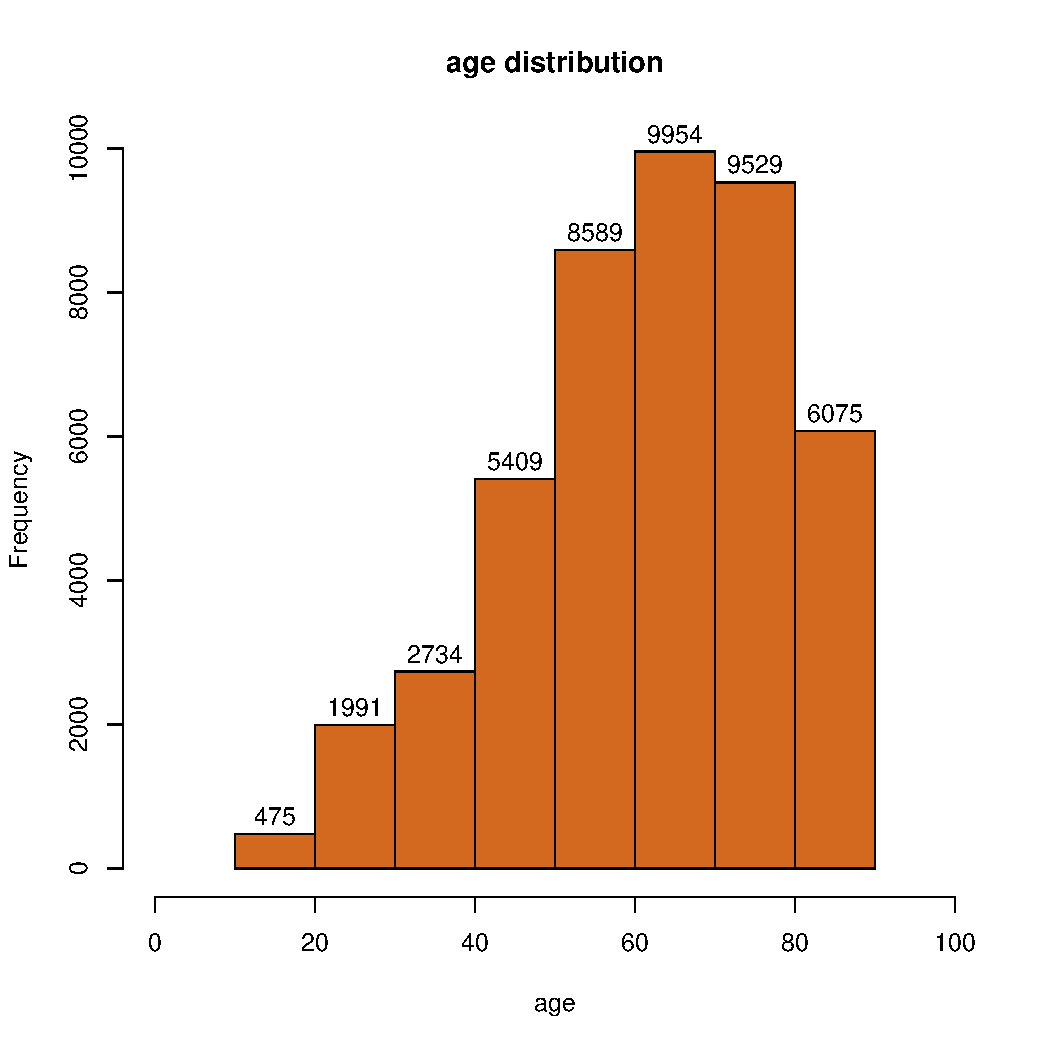
\includegraphics[width=0.6\linewidth]{img/age-distr}
		\caption{Age distribution of patients selected}
		\label{fig:age-distr}
	\end{figure}
	
\end{document}